\newpage
\subsection{Use case}

% \begin{figure}[!h]
%     \centering
%     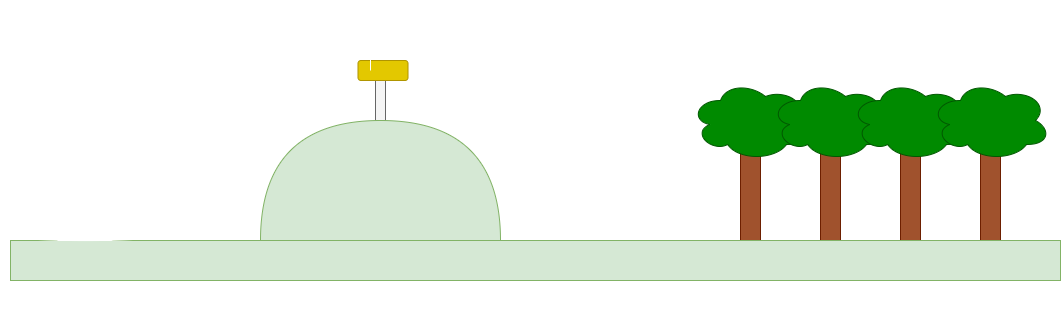
\includegraphics[width=1\textwidth]{\currfiledir/figures/use_case.png}
%     \caption{Use case of the system}
%     \label{fig:forest2}
% \end{figure}


The use case would be as following:
The researchers come once to install the system on a pole on a hill, in front of the group of trees they want to observe. The system would then be placed in the desired location within the forest. The system would be sending data to researchers to ensure that it is functioning properly and that the pictures being taken are of high quality. After 3 months, the researchers would return to the forest to retrieve the system, the stored pictures, and logs about the system state. Then, the researchers would be able to analyse the images.


\newpage
\begin{figure}[!h]
    \centering
    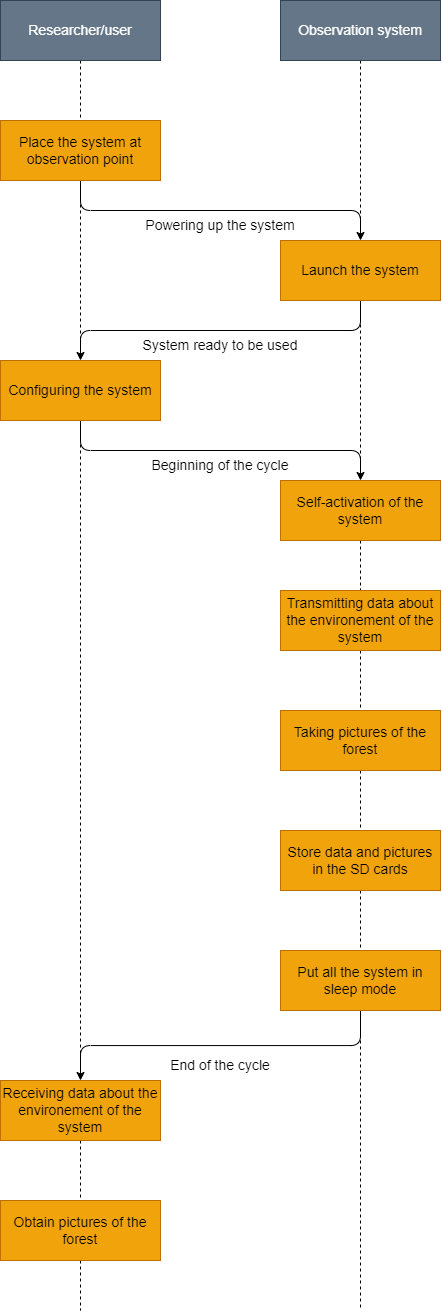
\includegraphics[height=0.95\textheight]{\currfiledir/figures/usage_scenario.png}
    \caption{Picture representing the intended usage scenario for the system.}
\end{figure}
